\newpage
\section{Schroedinger’s Equation}
A classical wave $\psi(x,y,z,t)$ satisfies the wave equation
\begin{align*}
    \frac{1}{v^2}\frac{\partial^2\psi}{\partial t^2}=\nabla^2\psi
\end{align*}

In the quantum theroy, a microscopic particle i described by a probability amplitude $\psi(x,y,z,t)$, and the probability of finding it is proportional to 
\begin{align*}
    P(x,y,z,t)=|\psi(x,y,z,t)|^2
\end{align*}

\subsection{Schroedinger’s Equation}
\subsubsection{Classical Particle}
Let us start with a pedagogical discussion on how to write down an equation that governs the quantum behavior of a free particle of mass $m$ represented by a wave 
\begin{align*}
    \psi(x,t)=e^{i(kx-\omega t)}
\end{align*}
For a free classical one-dimensional particle, on the other hand, the energy is 
\begin{align*}
    E=\frac{p^2}{2m}
\end{align*}

According to the de Broglie's hypothesis, we expect
\begin{align*}
    p=&\frac{h}{\lambda}=\hbar k=-i\hbar \frac{1}{\psi(x,t)}\frac{\partial \psi(x,t)}{\partial x}\\
    p^2=&-\hbar^2\frac{1}{\psi(x,t)}\frac{\partial^2 \psi(x,t)}{\partial x^2}
\end{align*}
Similarly, we expect
\begin{align*}
    E=hv=\hbar \omega=i\hbar \frac{1}{\psi(x,t)}\frac{\partial \psi(x,t)}{\partial x}
\end{align*}


So using wave function, the energy-momentum relation is 
\begin{align*}
    i\hbar\frac{1}{\psi(x,t)}\frac{\partial \psi(x,t)}{\partial x}=-\frac{\hbar^2}{2m}\frac{1}{\psi(x,t)}\frac{\partial^2 \psi(x,t)}{\partial x^2}
\end{align*}

In the presence of potential, e.g. a harmonic potential $U(x)=\frac{ax^2}{2}$, the classical relation is modified to 
\begin{align*}
    E=\frac{p^2}{2m}+U(x)
\end{align*}
where $E$ is a constant of motion, but $p$ is not. In the other words, a plane wave is not a solution any more. 

\subsubsection{Schroedinger’s Equation}
Schroedinger proposedthat the wave function $\psi(x,t)$ of a single particle moving around in 1D satisfies
\begin{align*}
    i\hbar\frac{\partial \psi(x,t)}{\partial t}=-\frac{\hbar^2}{2m}\frac{\partial^2 \psi(x,t)}{\partial x^2}+U(x,t)\psi(x,t)
\end{align*}
where $U(x,t)$ is the potential energy of the particle and $m$ is the mass of the particle.  

We can easily generalize it to higher dimensions. Note that \highlight{Schroedinger’s equation} is a postulate of quantum mechanics, not derived from classical physics.

In most cases we discuss, the potential energy $U=U(x)$ is \highlight{independent of time}. 

We can solve the Schroedinger equation by an ansatz $\psi(x,t)=\phi(x)e^{-iEt/\hbar}$. The wave function $\phi(x)$ satisfies
\begin{align*}
    \frac{\partial^2\phi(x)}{\partial x^2}+\frac{2m}{\hbar^2}[E-U(x)]\phi(x)=0
\end{align*}
The particular solutions are $e^{ikx}$ and $e^{-ikx}$, the general solution is the linear combination of two particular solutions. In free space, $U(x)=0$. The general solution is 
\begin{align*}
    \phi(x)=Ae^{ikx}+B^{-ikx}
\end{align*}
where A and B are constants and $k=\sqrt{2mE}/\hbar$. 

The complete time-dependent wave function is 
\begin{align*}
    \psi(x,t)=Ae^{i(kx-\omega t)}+Be^{-i(kx+\omega t)}
\end{align*}
where $\omega=E/\hbar$. The two terms correspond to right- and left-moving waves, respectively. 

Consider the right-moving wave $\psi(x,t)=Ae^{i(kx-\omega t)}$, the probability density is 
\begin{align*}
    |\psi(x,t)|^2=\psi^{\dagger}(x,t)\psi(x,t)=|A|^2
\end{align*}
That means that if we make a measurement to locate the particle, the location could turn out t be at any $x$ value. 

\subsection{Reflection from a Potential Step}
Consider a beam of nonrelativistic electrons, each o ftotal energy $E$, along an $x$ axis through a narrow tube. They experience a negative electric potential step of height $V_b<0$ at $x=0$. 

\begin{figure}[H]
    \centering
    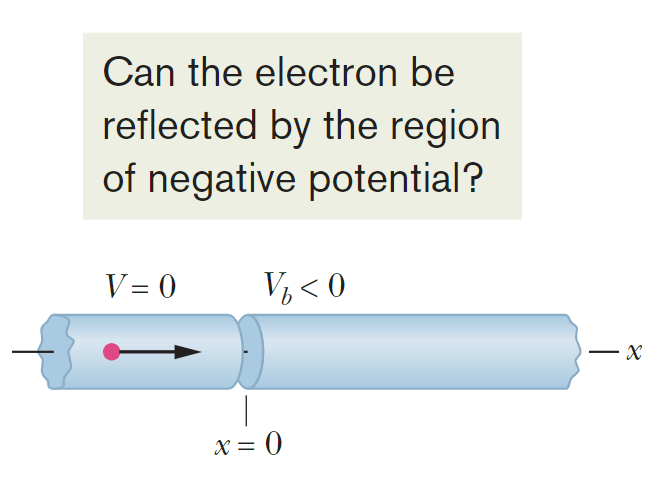
\includegraphics[width=0.229\textwidth]{Lec23/a beam of nonrelativistic electrons through a narrow tube}
    \caption{a beam of nonrelativistic electrons through a narrow tube}
\end{figure}

We consider the situation where $E>qV_b$. \highlight{Classically, electrons should all pass through the boundary}. Their total energy should be conserved, so their kinetic energy, hence speed, decreases when their potential energy increases. 

But in \highlight{quantum mechanically}, we apply\\ Schroedinger's equation to the two regions separately. The wave function should be consistent with each other at $x=0$, both in value and in slope (\highlight{boundary conditions}). 

\begin{figure}[H]
    \centering
    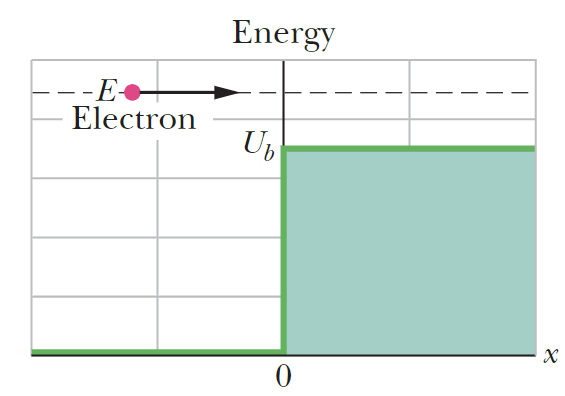
\includegraphics[width=0.309\textwidth]{Lec23/the two regions}
    \caption{the two regions}
\end{figure}

\begin{itemize}
    \item Region 1 $(x<0)$: $k=\sqrt{2mE}/\hbar$
    \begin{align*}
        \psi_1=Ae^{ikx}+Be^{-ikx}
    \end{align*}
    \item Region 2 $(x>0)$: $k_b=\sqrt{2m(E-qV_b)}/\hbar$
    \begin{align*}
        \psi_2=Ce^{ik_b x}+De^{-ik_b x}
    \end{align*}
\end{itemize}

We can first set $D=0$, because there is no electron source off to the right, and there can be no electrons moving to the left in region 2. We now consider boundary conditions at $x=0$:
\begin{align*}
    A+B=C &\text{ (matching of values)}\\
    Ak-Bk=Ck_b &\text{ (matching of slopes)}
\end{align*}

We should be able to solve $B/A$ and $C/A$, but not $A$, $B$ and $C$. Note that the absolute values are not important for our purpose (it can be related to the beam intensities, though). 

\subsubsection{Reflection and Transmission Coefficients}
Indeed, to find the probability that electrons reflect from the step, we need to relate the probability density of the reflected wave $(Be^{-ikx})$ to that of the incident wave $(Ae^{ikx})$. We thus define a reflection coefficient $R$: 
\begin{align*}
    R=\frac{|B|^2}{|A|^2}=\left|\frac{k-k_b}{k+k_b}\right|^2
\end{align*}
Quantum mechanically, electrons are reflected from the boundary, but only with a probability. 

Similarly, the transmission coefficient (the probability of transmission) is 
\begin{align*}
    T=1-R=\frac{4kk_b}{|k+k_b|^2}
\end{align*}

What inspires us to define $T$ in this way? Well, one can consider an alternative quantity
\begin{align*}
    \frac{|C|^2}{|A|^2}=\frac{4k^2}{|k+k_b|^2}=T\frac{k}{k_b}
\end{align*}

Recall current density $J=nqv$. Not surprisingly, one finds
\begin{align*}
    T=\frac{|C|^2 k_b}{|A|^2 k}=\frac{|C|^2 q(\hbar k_b /m)}{|A|^2 q(\hbar k/m)}=\frac{J_{transmitted}}{J_{incident}}
\end{align*}

One can also write 
\begin{align*}
    R=\frac{J_{reflected}}{J_{incident}}
\end{align*}

Therefore, $T=1-R$ is nothing but the conservation of current
\begin{align*}
    J_{transmitted}=J_{incident}-J_{reflected}
\end{align*}

\subsection{Tunneling through a Potential Barrier}
Now consider a potential energy barrier, which is a region of thickness $L$ where the electric potential is $V_b (<0)$ and the height is $U_b (=qV_b)$.

\begin{figure}[H]
    \centering
    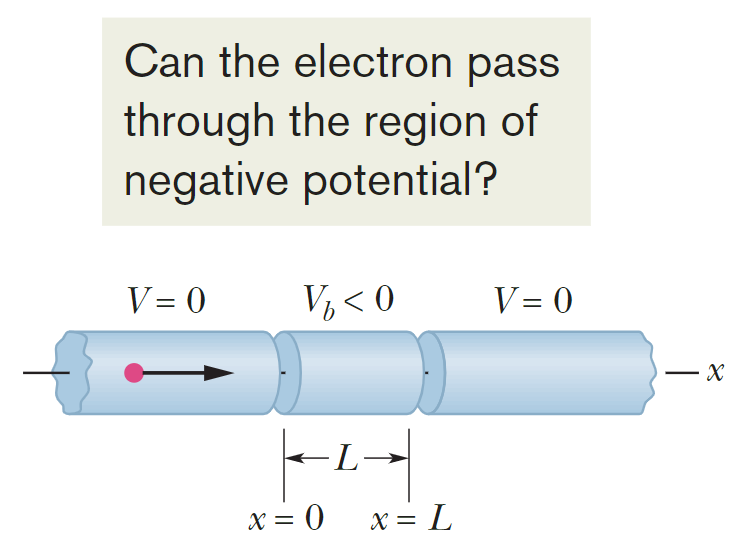
\includegraphics[width=0.309\textwidth]{Lec23/Tunneling through a Potential Barrier}
    \caption{Tunneling through a Potential Barrier}
\end{figure}

We consider the situtaion where $E<qV_b$. \highlight{Classically, electrons are forbidden in the barrier region, hence all reflected}. However, a matter wave, has a finite probability of leaking (or, better, tunneling) through the barrier and materializing on the other side. 

We are interested in the probability of the electron appearing on the other side of the barrier. Thus, we want the transmission coefficient $T$. The general procedure is the following. 

\begin{figure}[H]
    \centering
    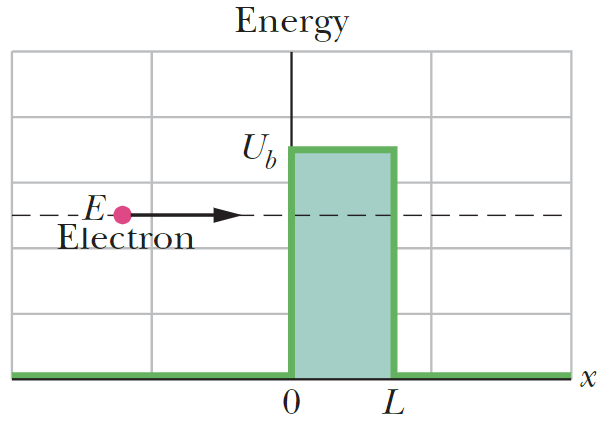
\includegraphics[width=0.309\textwidth]{Lec23/three regions}
    \caption{three regions}
\end{figure}

\begin{enumerate}
    \item Separate the space into three regions and solve Schroedinger's equation in each region (\highlight{$3\times 2-1=5$ unknowns}).
    \item Apply boundary conditions at the two boundaries (\highlight{$2\times 2=4$ equations}).
    \item Calculate the tunneling coefficient.
\end{enumerate}

We shall just examine the general results. 

\begin{enumerate}
    \item The oscillating curve to the left of the barrier (for $x<0$) is a combination of the incident matter wave and the reflected matter wave (which has a smaller amplitude than the incident wave). The oscillation occur because these two waves, traveling in opposite directions, interfere with each other, setting up a \highlight{standing wave pattern}. 
    \item Within the barrier (for $0<x<L$) the probability density \highlight{decreases exponentially} with $x$. However, if $L$ is small, the probability density is not quite zero at $x=L$. 
    \item To the right of the barrier (for $x>L$), the probability density plot describes a \highlight{transmitted wave} (through the barrier) with low but constant amplitude. 
\end{enumerate}

\begin{figure}[H]
    \centering
    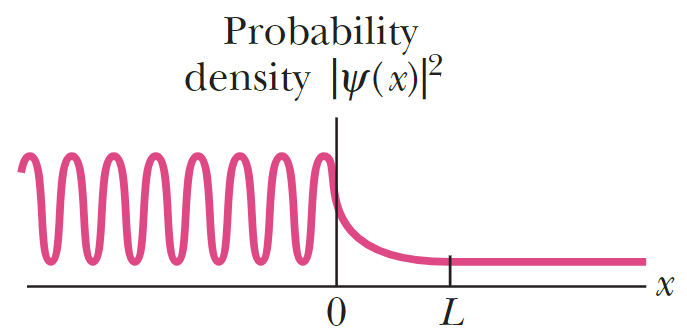
\includegraphics[width=0.309\textwidth]{Lec23/the general results}
    \caption{the general results}
\end{figure}

We can assign a transmission coefficient $T$ to the incident matter wave and the barrier. The transmission coefficient $T$ is approximately
\begin{align*}
    T\approx& e^{-2kL}\\
    \text{where } k=&\frac{\sqrt{2m(qV_b-E)}}{\hbar}
\end{align*}

The exact result can be obtained for any $U_b (=qV_b)$ and $L$. 

\begin{figure}[H]
    \centering
    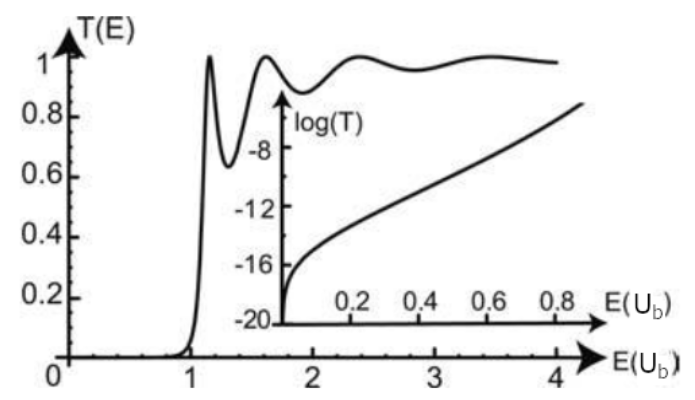
\includegraphics[width=0.309\textwidth]{Lec23/T and Ub}
    \caption{$T$ and $U_b$}
\end{figure}

In general, we speak of tunneling if $E<U_b$. In this regime, $T(E)$ increases approximately exponentially with energy, as shown in the inset. For $E\gg U_b$, $T(E)=1$ as expected classically. 

\subsection{Scanning Tunneling Microscope (STM)}
The size of details that can be seen in an optical microscope is limited by the wavelength of the light the microscope uses (about 300 nm for ultraviolet light). We use electron matter waves (tunneling through potential barriers) to create images on the atomic scale. A fine metallic tip, mounted on quartz rods, is placed close to the surface to be examined. The space between the surface and the tip forms a potential energy barrier.

\begin{figure}[H]
    \centering
    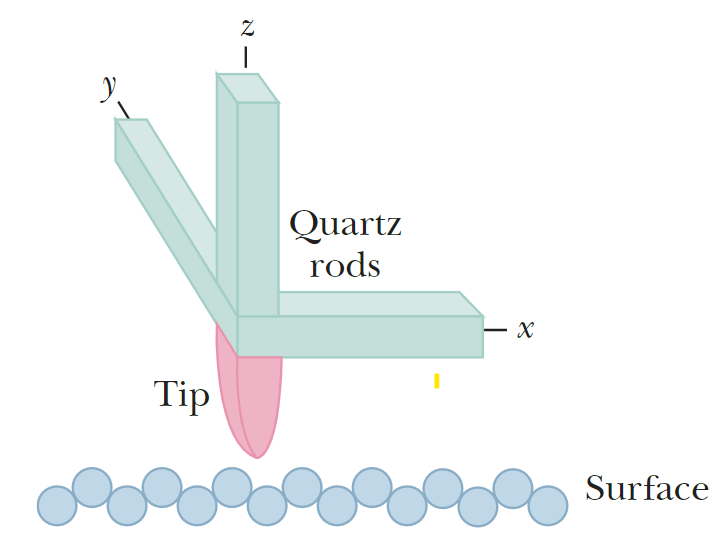
\includegraphics[width=0.309\textwidth]{Lec23/Scanning Tunneling Microscope}
    \caption{Scanning Tunneling Microscope}
\end{figure}

\begin{figure}[H]
    \centering
    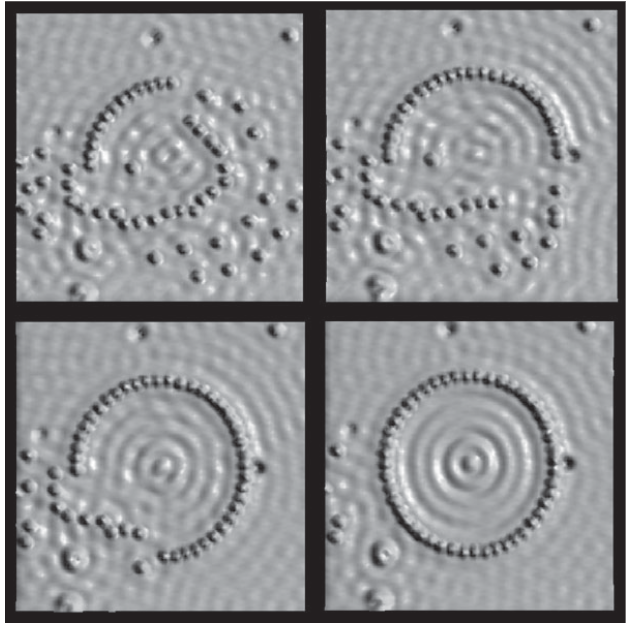
\includegraphics[width=0.309\textwidth]{Lec23/STM}
    \caption{An STM not only can provide an image of a static surface, it can also be used to manipulate atoms and molecules on a surface. }
\end{figure}

\subsection{Wave Packets}
What is the speed of a free quantum mechanical particle? The general solution of the particle is 
\begin{align*}
    \psi(x)=Ae^{ikx}+Be^{-ikx}, \, k=\sqrt{2mE}/\hbar
\end{align*}
or with standard time dependence, $e^{-i\omega t}, \, \omega=E/\hbar$
\begin{align*}
    \psi(x,t)=Ae^{i(kx-\omega t)}+Be^{-i(kx+\omega t)}
\end{align*}
The formula represents a right- and a left-moving wave with speed (of the wavefront)
\begin{align*}
    v_{qh}=\frac{\omega}{k}=\frac{E}{k\hbar}=\sqrt{\frac{E}{2m}}
\end{align*}

On the other hand, the classical speed of a free particle with energy $E$ is given by 
\begin{align*}
    v_{cl}=\sqrt{\frac{2E}{m}}=2v_{qh}
\end{align*}

There are some Problems:
\begin{enumerate}
    \item The quantum mechanical wave function travels at \highlight{half the speed} of the particle it is sipposed to represent. 
    \item How to normalize the wave function of the free particle, say, represented by $Ae^{ikx}$? 
    \begin{align*}
        \int_{\infty}^{\infty}|\psi(x)|^2\,\mathrm{d}x=|A|^2\int_{\infty}^{\infty}1\,\mathrm{d} x=|A|^2\infty
    \end{align*}
    This wave function is \highlight{not normalizable}. 
\end{enumerate}

Apparently, the stationary (separable) solution don't represent physically realizable states; there is no such thing as a free particle with a definite energy. 

In quantum theory, a localized particle is modeled by a linear superposition of these stationary free-particle (or plane-wave) states.

\begin{figure}[H]
    \centering
    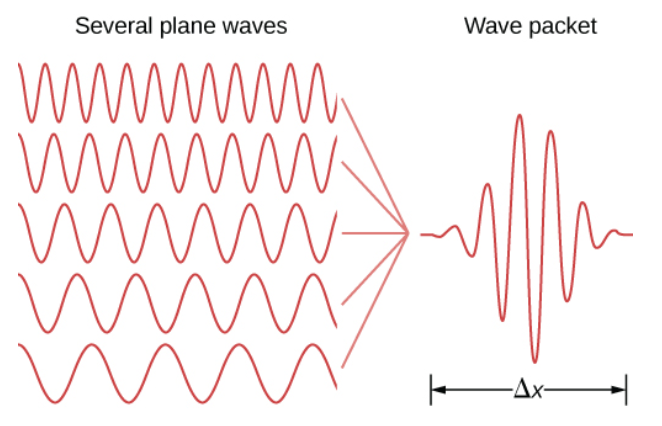
\includegraphics[width=0.309\textwidth]{Lec23/a localized particle}
    \caption{a localized particle}
\end{figure}

In general, we can construct a linear combination (integral over continuous $k$)
\begin{align*}
    \Psi (x,t) =\frac{1}{\sqrt{2\pi}}\int_{\infty}^{\infty}\phi(k)e^{i\left( kx-\omega t \right)}\, \mathrm{d}k
\end{align*}
This wave function can be normalized for appropriate $\phi(k)$. We call it a \highlight{wave packet}, which carries a range of $k$ and, hence, a range of energies and speeds. In a general quantum problem, we are given $\Psi(x,0)$ and needed to find $\Psi(x,0)$. The particle can be better localized ($\Delta x$ can be decreased) if more plane-wave states of different wavelengths or momenta are added together in the right way ($\Delta p$ is increased). According to Heisenberg, these uncertainties obey 
\begin{align*}
    \Delta x\Delta p \ge \frac{\hbar}{2}
\end{align*}

It turns out that the group velocity of the wave packet, not the phase velocity of the stationary states, matches the classical particle velocity.